% Generated from tex/chapters/ch04/08_構築技術.tex for the SWEBOK structure tree
\subsubsection{表明、契約による設計、防御的プログラミング}

表明とは、プログラム中に置かれる実行可能な条件式である。プログラムが想定する前提や不変条件が成り立っているかを実行時に確認する。開発時には欠陥を早く見つける助けになる。

契約による設計とは、各関数やクラスについて、呼び出し前に満たすべき事前条件、呼び出し後に保証する事後条件、常に守られる不変条件を明確にする考え方である。これにより、部品同士の責任範囲が明確になる。

防御的プログラミングとは、不正な入力や想定外の状態から関数を守るために、入力値を検査し、異常な場合の処理を決めることである。防御的に書くことで、欠陥の影響を局所化しやすい。

\begin{figure}[htbp]
\centering
\IfFileExists{assets/fig-ch04-09.png}{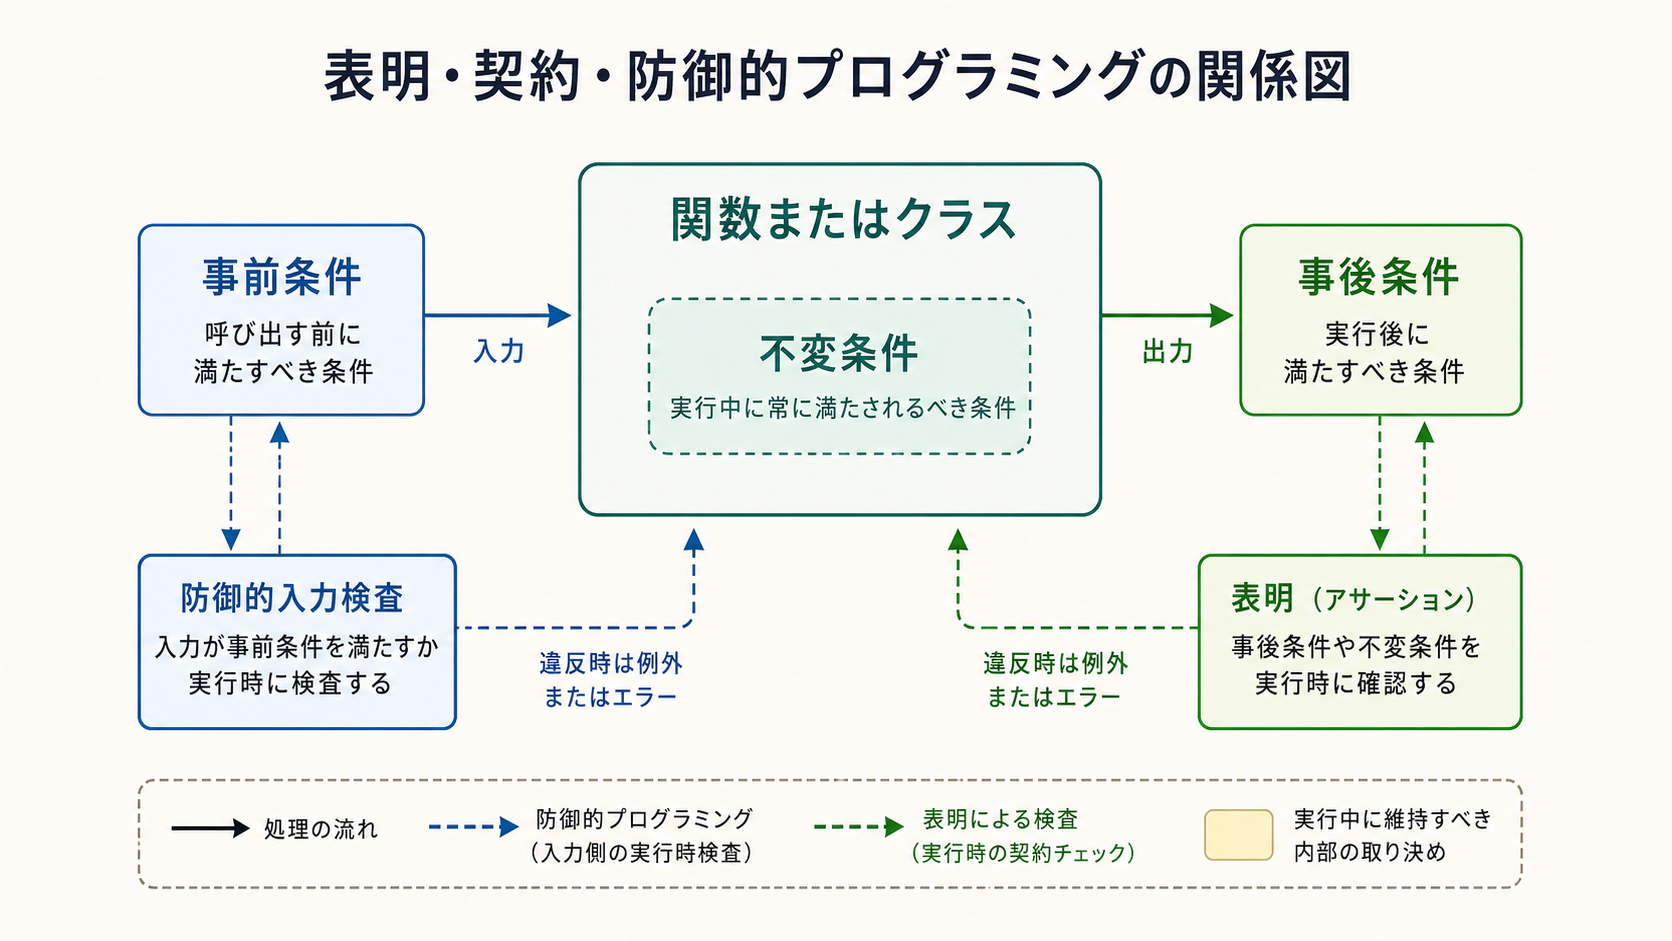
\includegraphics[width=0.96\linewidth]{assets/fig-ch04-09.png}}{\fbox{\parbox[c][48mm][c]{0.9\linewidth}{\centering 画像生成待ち\\表明・契約・防御的プログラミングの関係図}}}
\caption{表明・契約・防御的プログラミングの関係図}
\label{fig:ch04-09}
\end{figure}
